\documentclass[main]{subfiles}

\begin{document}
\section{Databehandling}
\subsection{Modul et}
Som benævnt i \cref{dataopsamling1} er der opsamlet data med afstanden $d$ som funktion af $f_s$. Der er taget tre målinger af afstanden $d$, pr. frekvens som varieres fra $120$ til $280 \ \si{\mega\hertz}$ med spring af 10 $\si{\mega\hertz}$ mellem hver måling. Grunden til de tre målinger pr. frekvens er for at komme tættere på en sand værdi med usikkerheder for hvert punkt, som her er valgt til at være standardafvigelsen på de tre målinger, altså således at $sds_{std} = \text{std}$. Målingspunkterne som ses på \cref{fig:rawdata_modul1} har centrum i gennemsnitsværdien af de tre målinger. Ydermere er tillagt en usikkerhed i målinger med lineal på
$ sds_{lin} = 1 \si{\milli\meter} $ . Altså er de endelige usikkerheder som ses på \cref{fig:rawdata_modul1}:  $ sds_{tot} = sds_{std} + sds_{lin} $.
\begin{figure}[H]
    \centering
    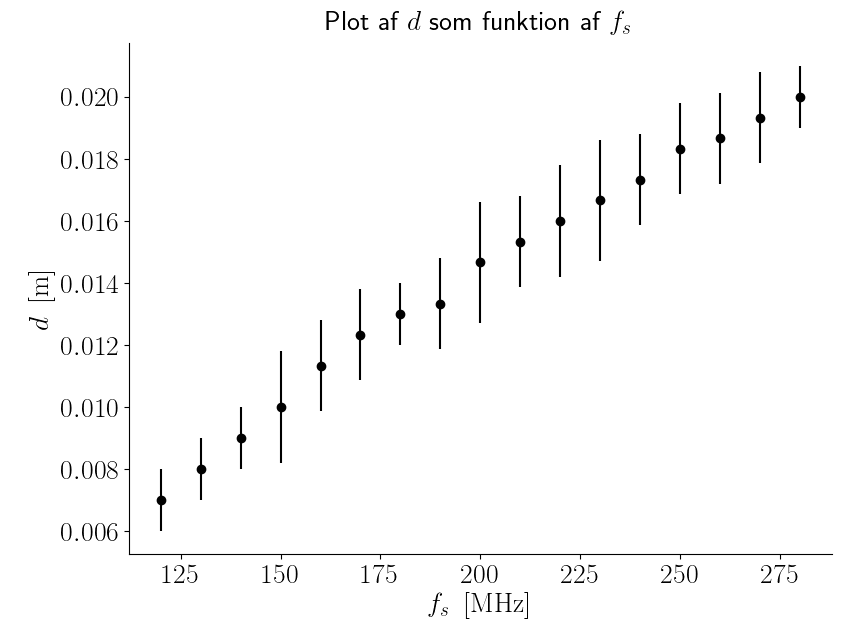
\includegraphics[width=\linewidth]{tegninger/rawdata_modul1.png}
    \caption{}
    \label{fig:rawdata_modul1}
\end{figure}
Idet at vi nu kender afstanden fra AOM'en ud til skærmen og afstanden fra $0^{th}$ ordens-pletten ud til $1^{st}$ ordens-pletten, kan vi nu finde vinklen $\theta_{sep}$ ved ?????\cref{eq:LURITS}.?????%%TODO indsæt formel i teori og cref her
Dette muliggør at afbilde $\theta_{sep}$ som funktion af $f_s$ hvilket er relevant da vi kan fitte til denne og gennem fittet ekstrahere lydens hastighed i krystallen ved ???\cref{eq:THETA = LAMBDA*FS/V_S}???. %TODO indsæt formel i teori og cref her
På figur \cref{fig:graf1} ses $\theta_{sep}$ plottet som funktion af $f_s$, med indlagt fit på data. Usikkerhederne på denne graf er bestemt ved ophobningsloven idet at usikkerhederne på $l$ og $d$ er kendte.
%TODO vurder om vi lige skal vise udregningen af usikkeden her
\begin{figure}[H]
    \centering
    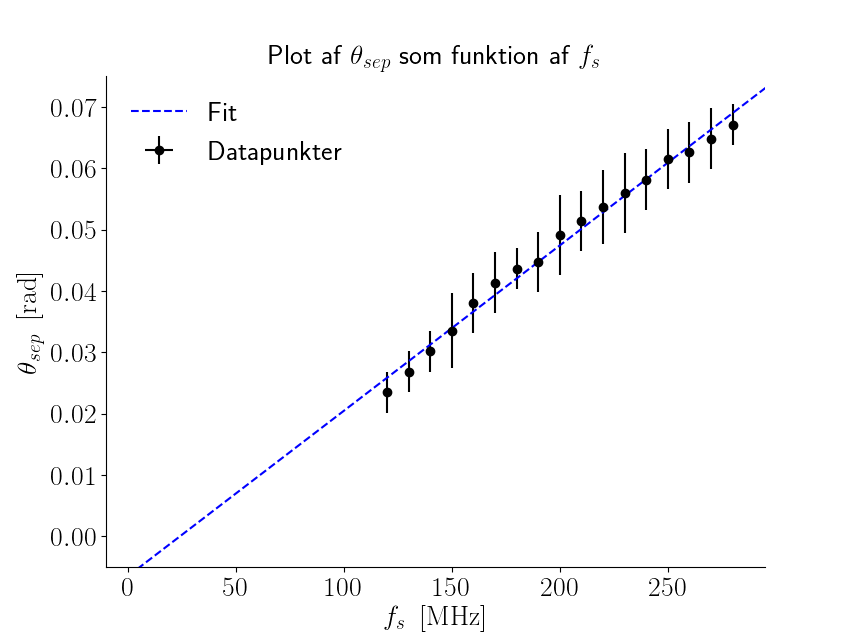
\includegraphics[width=\linewidth]{tegninger/graf1.png}
    \caption{}
    \label{fig:graf1}
\end{figure}
Det ses på \cref{fig:graf1} at den fittede kurve ikke skærer i $(0,0)$, hvilket den burde grundet udtrykket i \cref{eq:THETA = LAMBDA*FS/V_S}.%TODO indsæt formel i teori og cref her
Ydermere ses det at linjen skærer datapunkterne indenfor deres usikkerhedsfaner.Det ses fra \cref{eq:sep} at hældningen, $k_{hældning}$ på linjen bliver $ k_{hældning} = \frac{\lambda_L}{v_S}$, og da $k_{hældning} = \SI{0,213}{\second}$ kan finde lydens hastighed i krystallen til at være:
\begin{equation}
  \nonumber v_S = \frac{\lambda_L}{k_{hældning}} = 3376,9
\end{equation}


%TODO Lav statistik her

\begin{figure}[H]
    \centering
    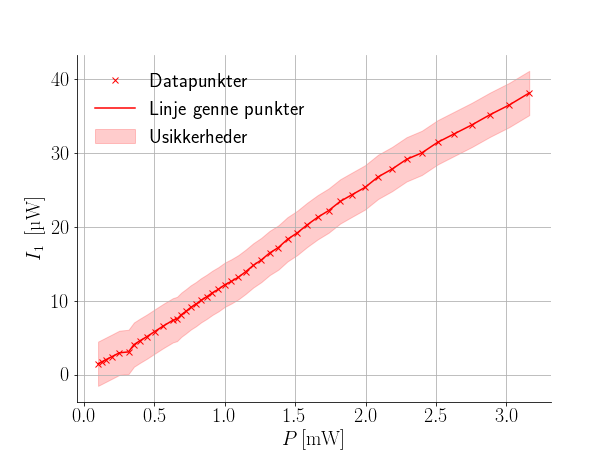
\includegraphics[width=\linewidth]{tegninger/graf2.png}
    \caption{}
    \label{fig:graf2}
\end{figure}




\end{document}
